\section{Results}
\label{sec:results}

We conducted qualitative and quantitative performance evaluations of \emph{autoreject} using four different datasets comparing it to a baseline condition without rejection as well as three different alternative artifact rejection procedures.

\subsection{Peak-to-peak thresholds}

\begin{figure}[htb!]
	\centering
	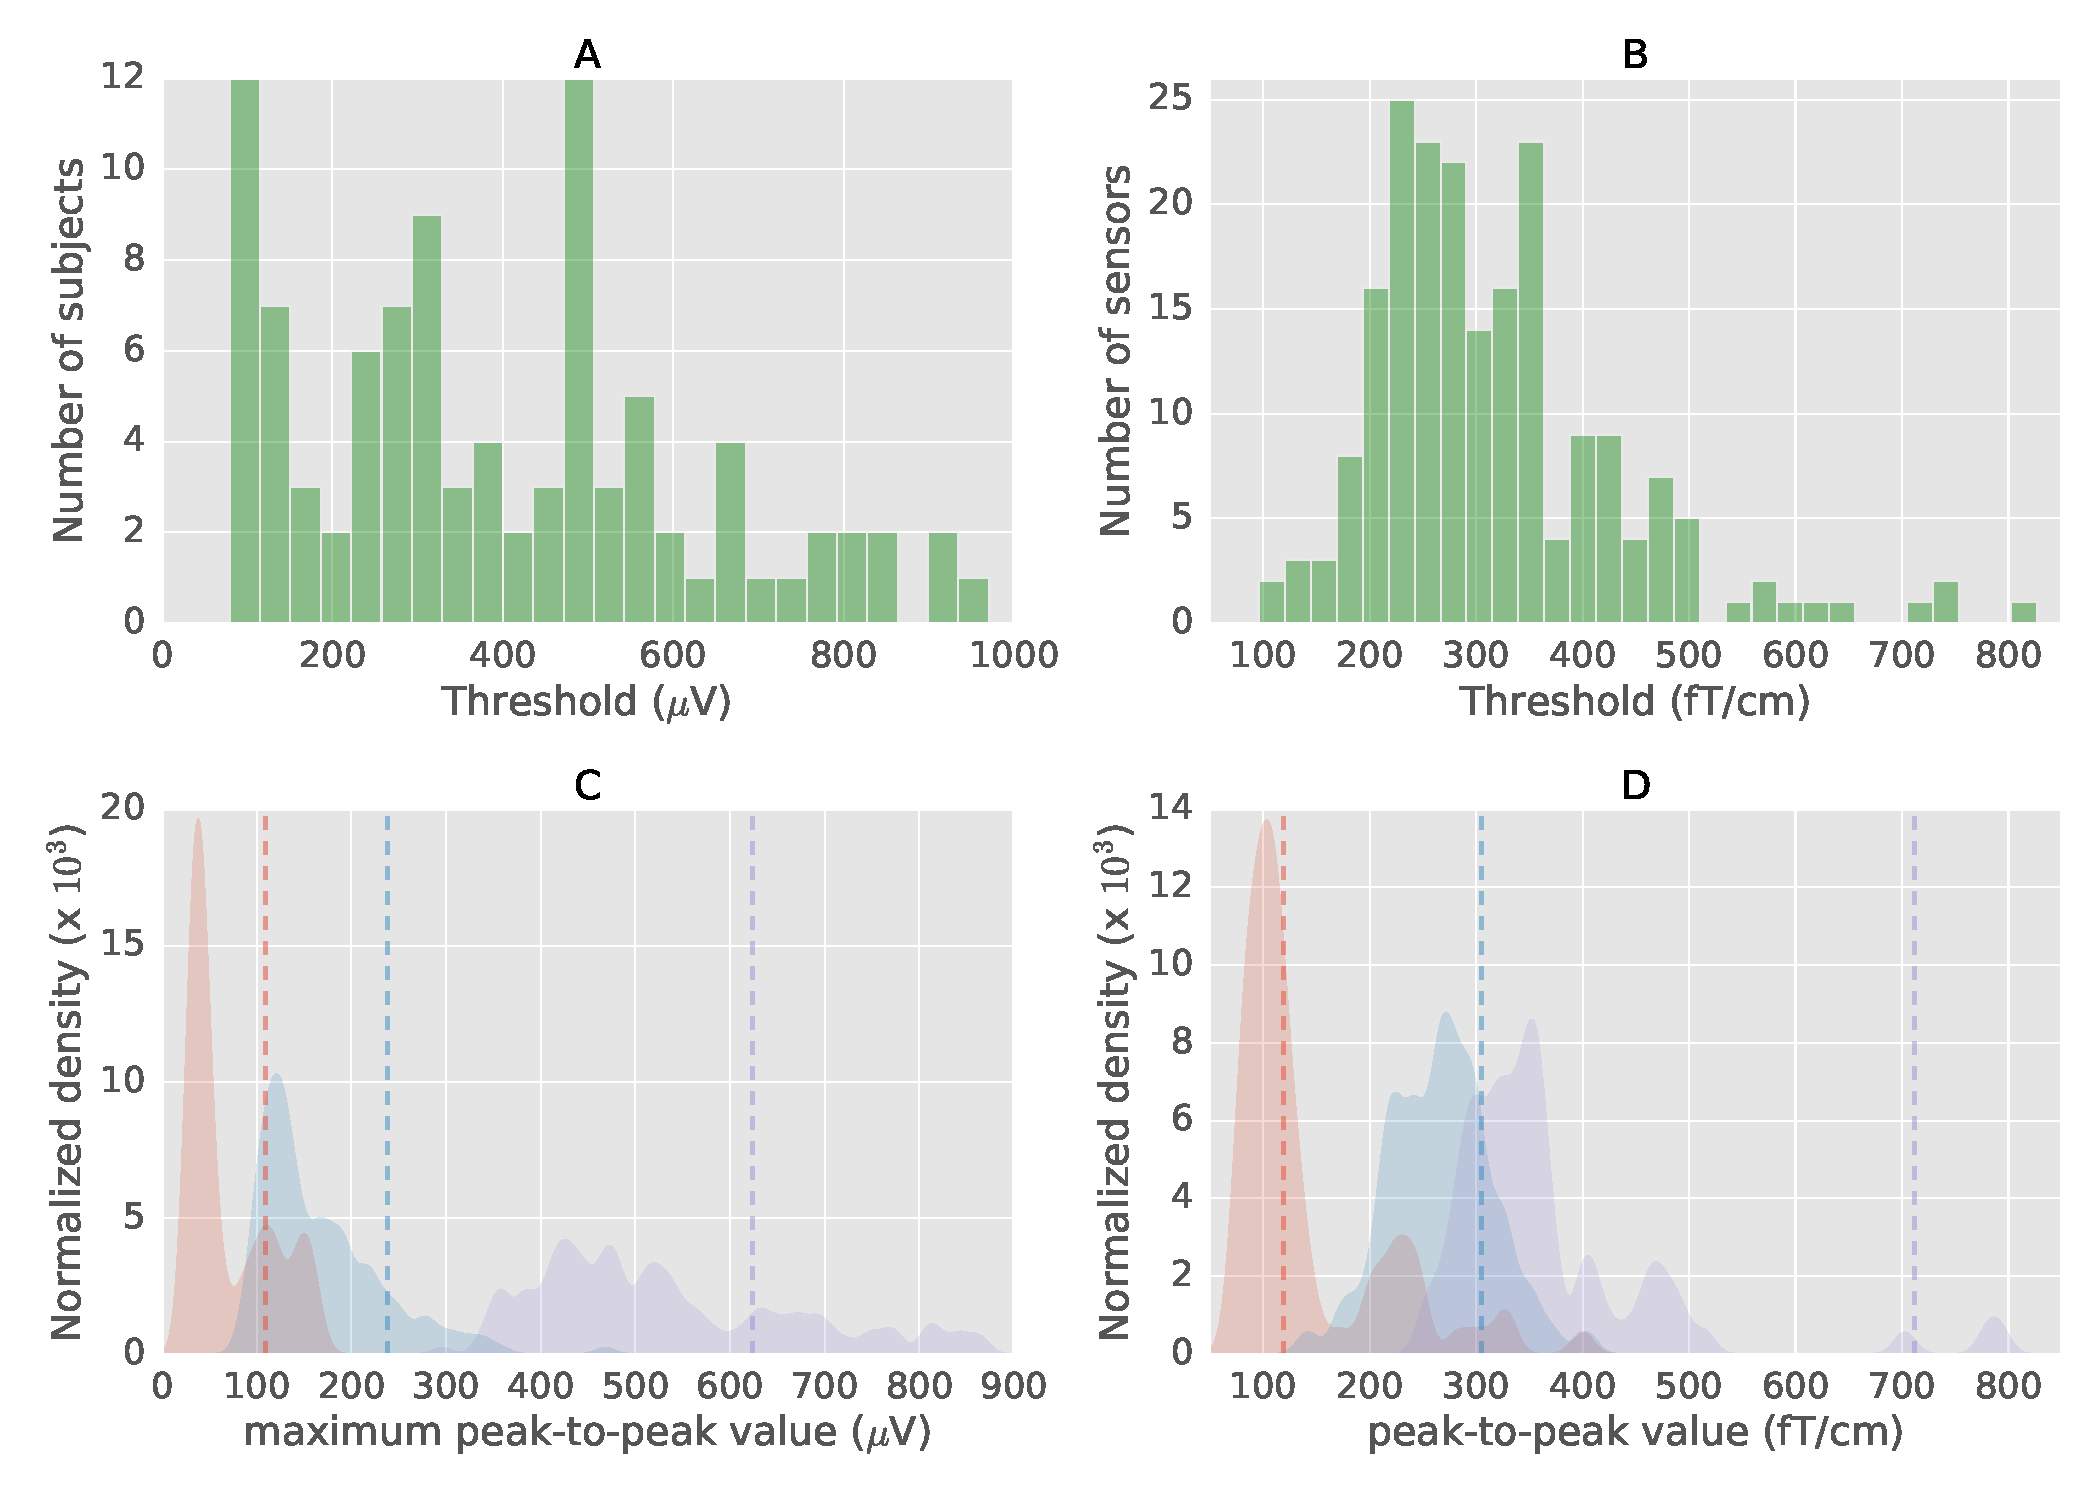
\includegraphics[width=0.9\linewidth]{figures/figure6.pdf}
    \caption[Histograms and kernel density plots of peak-to-peak thresholds.]{A. Histogram of thresholds for subjects in the EEGBCI dataset with \emph{autoreject (global)} B. Histogram of sensor-specific thresholds in gradiometers for the MNE sample dataset (Section~\ref{sec:results}). C. Normalized kernel density plots of maximum peak-to-peak value across sensors for three subjects in the EEGBCI data. Vertical dashed lines indicate estimated thresholds. Density plots and thresholds corresponding to the same subject are the same color. D. Normalized Kernel Density plots of peak-to-peak values for three MEG sensors in the MNE sample dataset. The threshold indeed has to be different depending on the data (subject and sensor).}
    \label{fig:hist}
\end{figure}

First, let us convince ourselves that the peak-to-peak thresholds indeed need to be learned. In Figure~\ref{fig:hist}A, we show a histogram of the thresholds learned on subjects in the EEGBCI dataset using \emph{autoreject (global)}. This figure shows that thresholds vary a lot across subjects. One could argue that this is due to variance in the estimation process. To rule out such a possibility, we plotted the distribution of maximum peak-to-peak thresholds as kernel density plots in Figure~\ref{fig:hist}C for three different subjects. We can see that these distributions are indeed subject dependent, which is why a different threshold must be learned for each subject. In fact, if we were to use a constant threshold of $150 \mu{V}$, in $17\%$ of the subjects, all the trials would be dropped in one of the two conditions. Of course, from Figure~\ref{fig:hist}A, we can now observe that $150 \mu{V}$ is not really a good threshold to choose for many subjects.
%

We show here the maximum peak-to-peak amplitude per sensor because this is what decides if a trials should be dropped or not in the case of \emph{autoreject (global)}. Note that, if instead, we examined the distribution of peak-to-peak amplitudes across all sensors and trials, we would see a quasi-normal distribution. When all the sensors are taken together, a ``smoothing" effect is observed in the distribution. This is a consequence of the central limit theorem. This also explains why we cannot learn a global threshold using all the peak-to-peak amplitudes across trials and sensors.

With the \emph{autoreject (local)} approach, a threshold is estimated for each sensor separately. The histogram of thresholds for the MNE sample dataset is plotted in Figure~\ref{fig:hist}B. It shows that the threshold varies even across homogeneous MEG sensors. Figure~\ref{fig:hist}D shows the distribution of peak-to-peak thresholds for three different MEG sensors. This graph confirms actual sensor-level differences in amplitude distributions, which was also previously reported in the literature~\citep{junghofer2000statistical}. With this work, we go one step further by learning automatically the thresholds in a data-driven way rather than asking users to mark them interactively.

\begin{figure}[htb!]
	\centering
	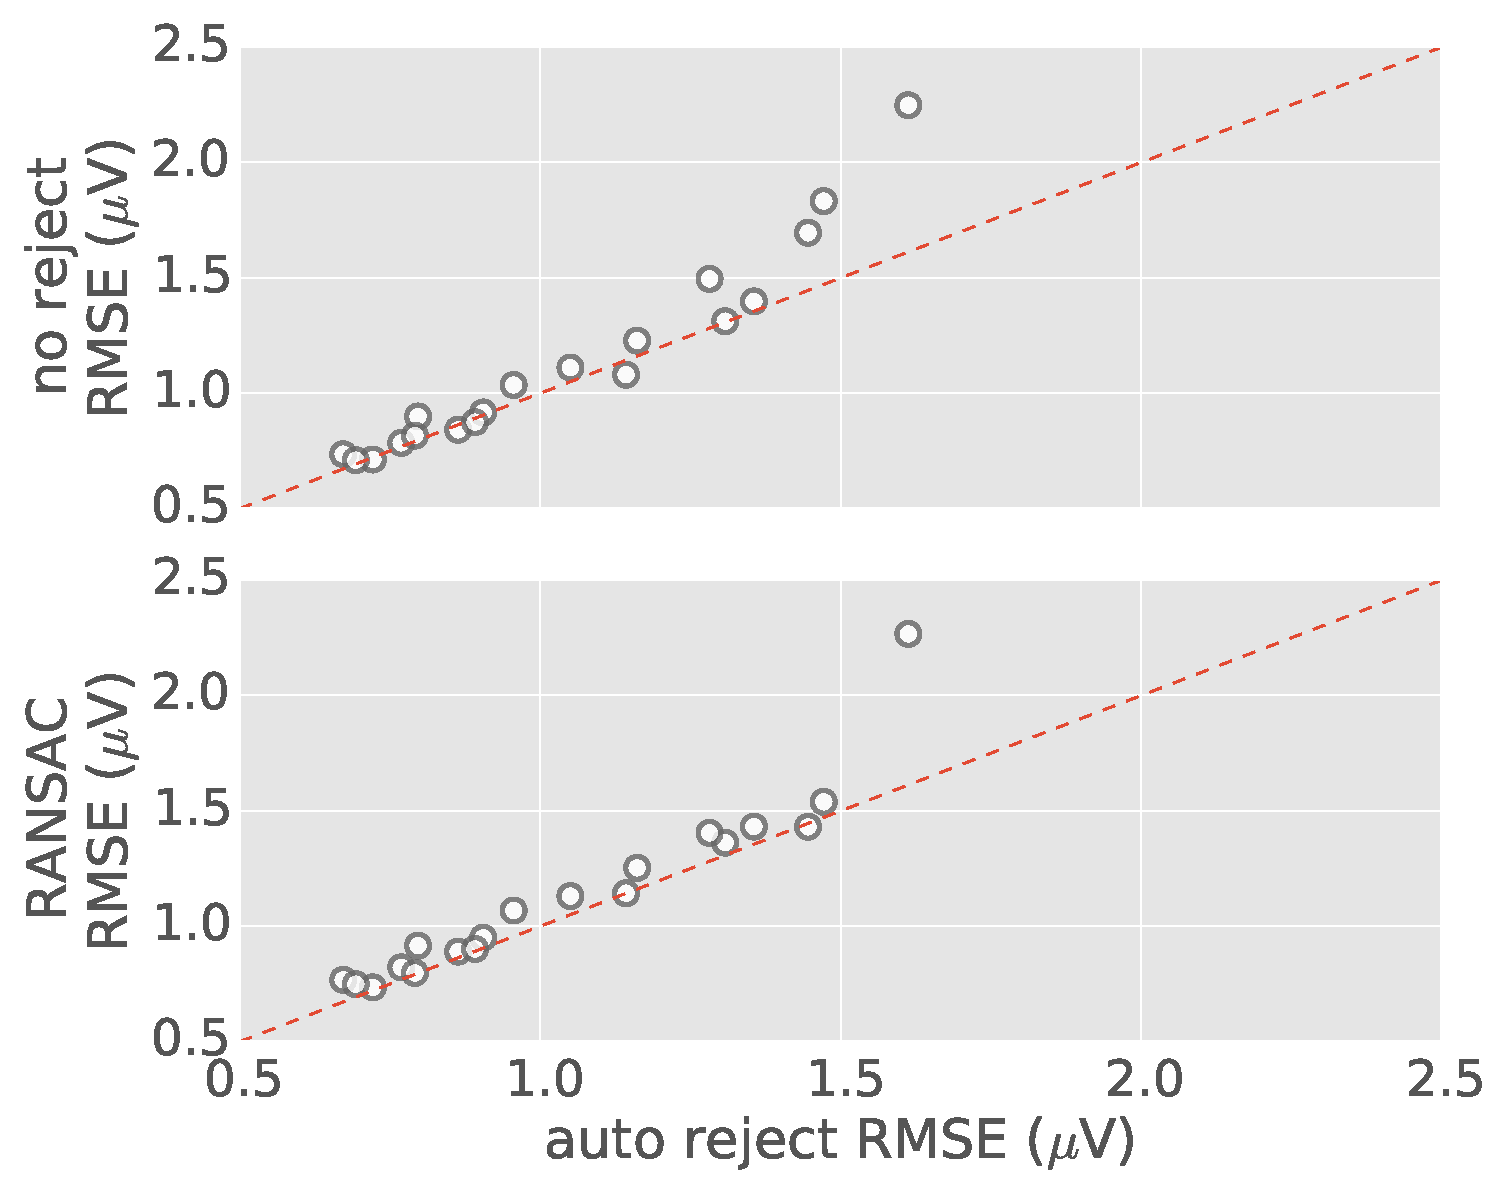
\includegraphics[width=0.8\linewidth]{figures/figure5.pdf}
    \caption[The evoked response (average of data across trials) on three different datasets before and after applying \emph{autoreject}]{The evoked response (average of data across trials) on three different datasets before and after applying \emph{autoreject} --- the MNE sample data, the HCP data and the EEG faces data. Each sensor is a line on the plots. On the left, manually annotated bad sensors are shown in red. The algorithm finds the bad sensors automatically and repairs them for the relevant trials. Note that it can even fix multiple sensors at a time and works for different modalities of data acquisition.}
    \label{fig:sample_evoked}
\end{figure}

\subsection{Visual quality check}

\begin{figure}[htb!]
    \centering
    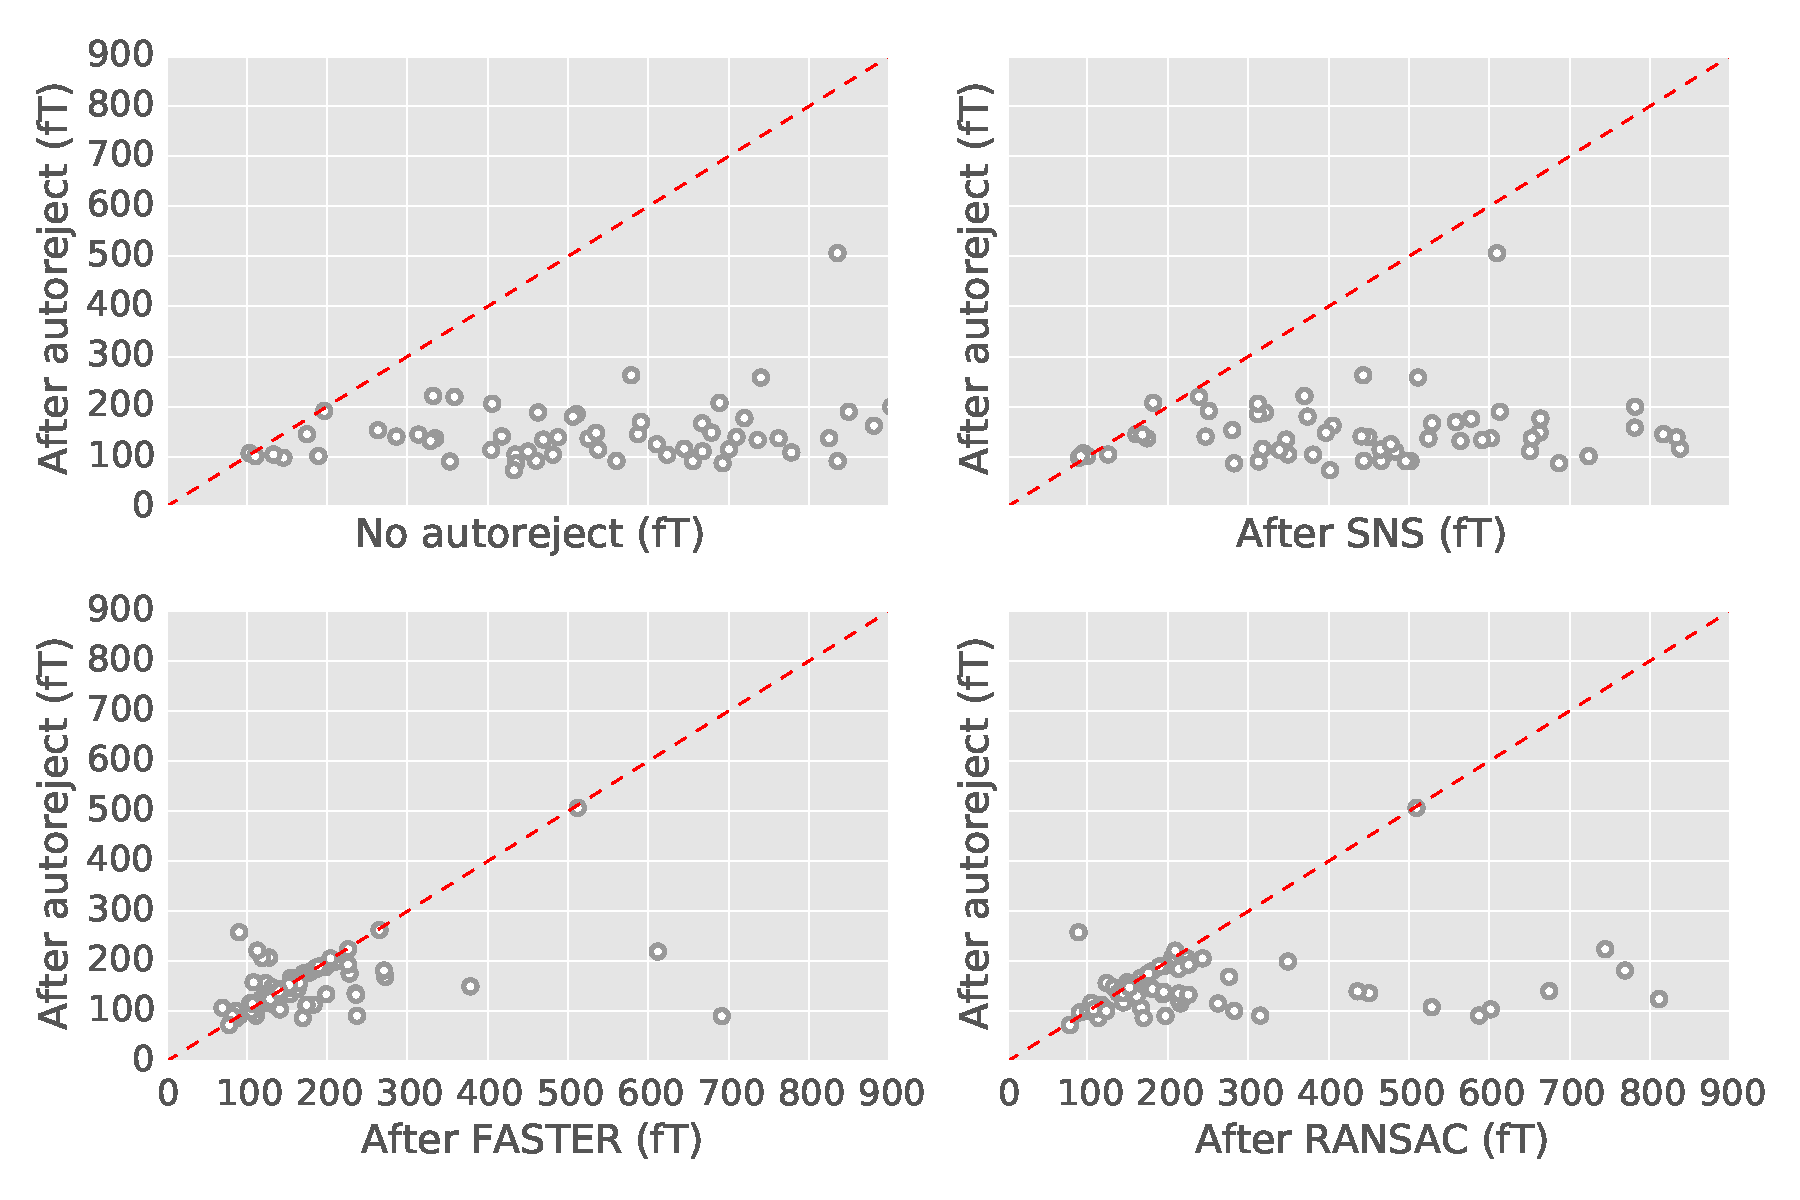
\includegraphics[width=0.75\linewidth]{figures/figure4.pdf}
    \caption[Scatter plots for the results with the HCP data.]{Scatter plots for the results with the HCP data. For each method, the $\infnorm{\cdot}$ norm of the difference between the HCP ground truth and the method is taken. Each circle is a subject. (A) \textit{autoreject (local)} against no rejection, (B) \textit{autoreject (local)} against Sensor Noise Suppression (SNS) (SNS), (C) \textit{autoreject} against FASTER, (D) \textit{autoreject (local)} against RANSAC. Data points below the dotted red line indicate subjects for which \textit{autoreject (local)} outperforms the alternative method.}
    \label{fig:hcp_scatter}
\end{figure}

\begin{figure}[htb!]
    \centering
    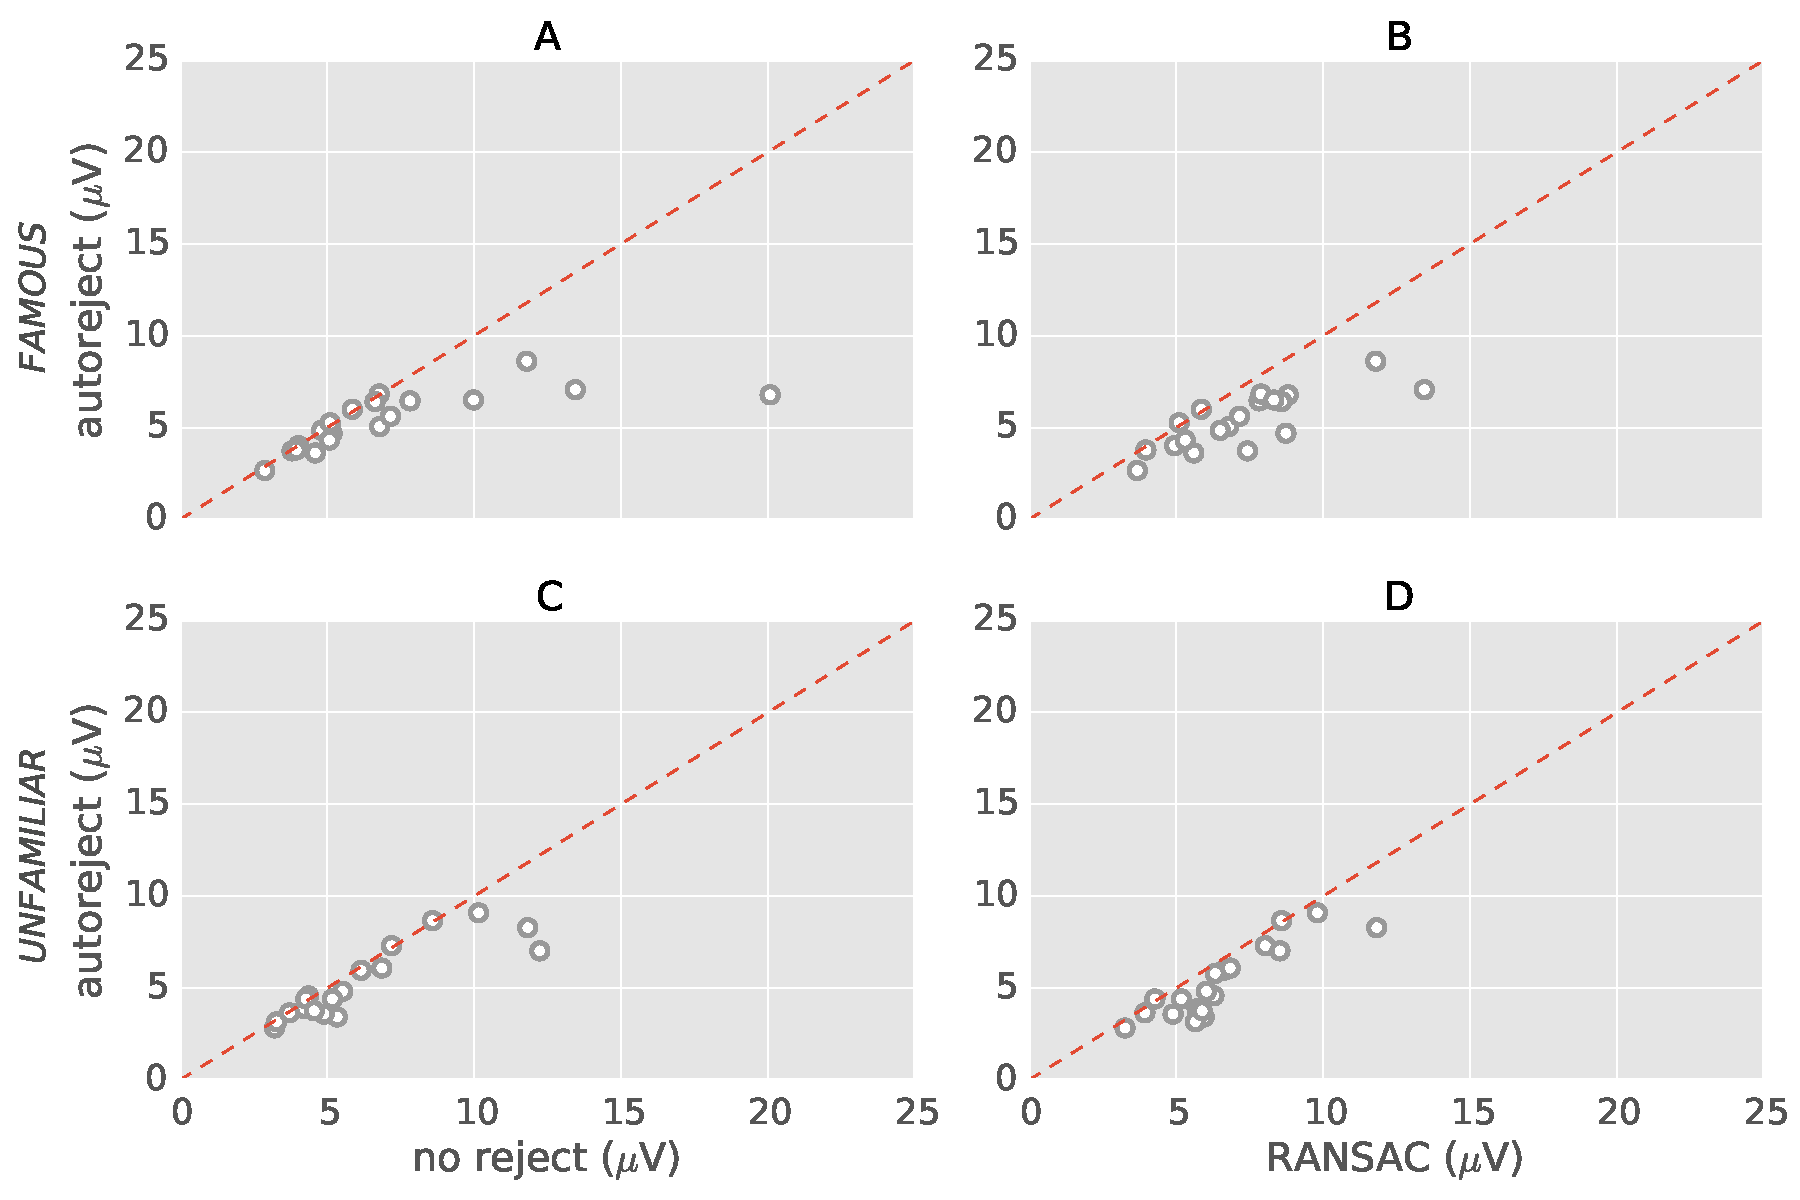
\includegraphics[width=0.75\linewidth]{figures/figure7.pdf}
    \caption[Scatter plots for the results with the 19 subjects from Faces dataset.]{Scatter plots for the results with the 19 subjects from Faces dataset. The first row (A) and (B) is for the condition ``famous" and the second row (C) and (D) is for the condition ``unfamiliar" faces. For each method, the $\infnorm{\cdot}$ norm of the difference between the ground truth and the estimates is computed. Each circle is a subject. Data points below the dotted red line indicate subjects for which \textit{autoreject (local)} outperforms the alternative method.}
    \label{fig:dgw_scatter}
\end{figure}

The average response plotted in a single graph, better known as ``butterfly plots'', constitutes a natural way to visually assess the performance of the algorithm for three different datasets -- MNE sample data, HCP MEG data, and EEG faces data. In Figure~\ref{fig:sample_evoked}, the subplots in the left column show the evoked response with the bad sensors marked in red. Right subplots, show data after applying the \emph{autoreject (local)} algorithm, with the repaired bad sensors in red. The algorithm works for different acquisition modalities -- MEG and EEG, and even when multiple sensors are bad. A careful look at the results, show that \emph{autoreject (local)} does not completely remove eyeblinks in the data as some of the blinks are time-locked to the evoked response. We will later discuss (Section~\ref{sec:discussion}) the possible solutions of applying ICA-based artifact correction in combination with \emph{autoreject (local)}.

\subsection{Quantification of performance and comparison with state-of-the-art}
\label{sec:benchmark_sensors}

We now compare these algorithms to \emph{autoreject (local)} using the data quality metric defined in Equation~\eqref{eq:infnorm}. We are interested not only in how the algorithms perform on average but at the level of individual subjects. To detail single subject performance, we present the data quality as scatter plots where each axis corresponds to the performance of a method. Figure~\ref{fig:hcp_scatter}, contains results on the HCP MEG data. We can observe from the top-left subplot of the figure that \emph{autoreject (local)} does indeed improve the data quality in comparison to the \emph{no rejection} approach. In Figure~\ref{fig:hcp_scatter}B, \emph{autoreject (local)} is compared against SNS. The SNS algorithm focuses on removing noise isolated on single sensors. Its results can be affected by the presence of multiple bad sensors and globally bad trials. This explains why \emph{autoreject (local)} outperforms SNS is this setting. In Figure~\ref{fig:hcp_scatter}C, we compare against FASTER. Even though \emph{autoreject (local)} is slightly worse than FASTER for a few subjects, FASTER is clearly much worse than \emph{autoreject (local)} for at least 3 subjects, and \emph{autoreject (local)} yields therefore less errors on average. Finally, Figure~\ref{fig:hcp_scatter}D shows comparison to RANSAC. In the PREP implementation, this algorithm is not fully data-driven in the classic sense of RANSAC. This is due to the fact that the inlier model is not learned but rather derived from the physics of the interpolation. It is therefore an algorithm which is conceptually close to \emph{autoreject}. However, a critical difference is that the parameters of this method still need to be tuned. This can be a problem as these parameters can be suboptimal on some datasets. Some experiments showed that it is for example the case for the EEG faces data, where it is possible to obtain better results by manually tuning the RANSAC parameters, rather than using the values proposed by the original authors.

Figure~\ref{fig:dgw_scatter} presents scatter plots for the EEG faces data.
%
Here, we restrict our comparison to RANSAC as it is conceptually the closest to \emph{autoreject}. On this data, we apply the algorithms on both the conditions -- famous and unfamiliar faces. It should be noted that the ground truth for this data was generated automatically with no additional annotations from human experts. However, a sanity check was performed on the ground truth by visual inspection. Here too, \emph{autoreject} offers good results across all subjects, and even for the subjects for which RANSAC underperforms.

\clearpage
\begin{sidewaysfigure}
	\centering
	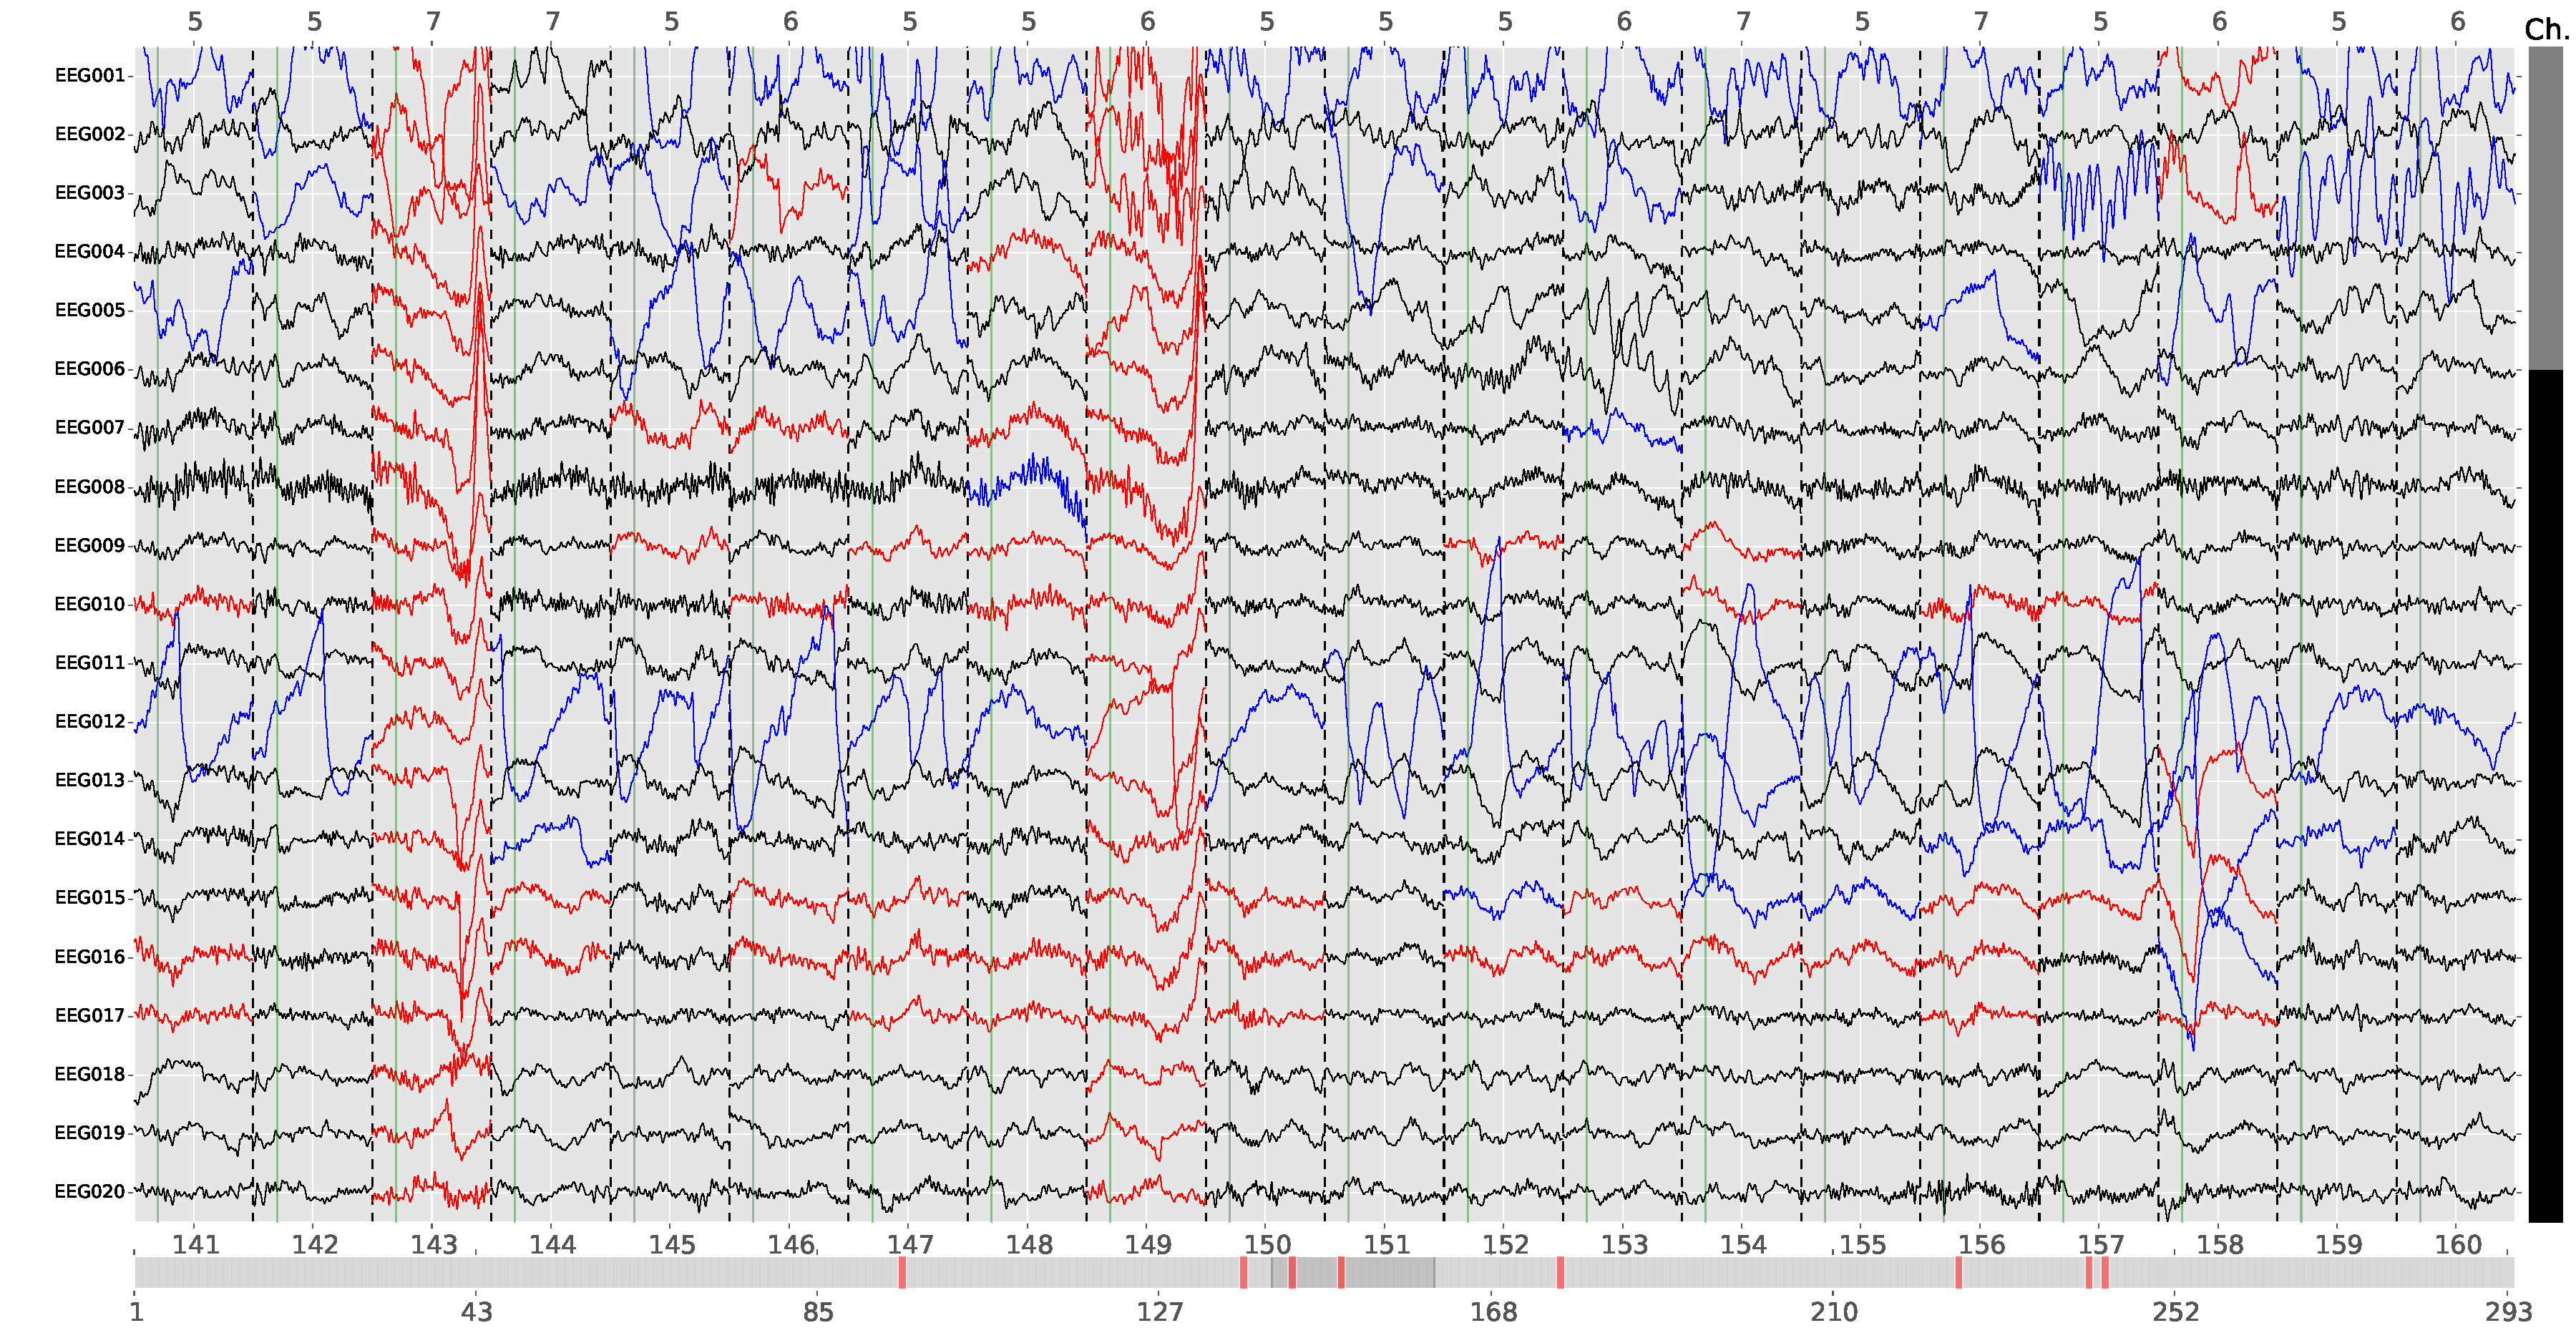
\includegraphics[width=\textwidth]{figures/figure8.pdf}
    \caption[An example diagnostic plot from an interactive viewer with \emph{autoreject (local)}]{An example diagnostic plot from an interactive viewer with \emph{autoreject (local)}. The data plotted here is subject 16 for the condition `famous' in the EEG faces data. Each row is a different sensor. The trials are concatenated along the x axis with dotted vertical lines separating consecutive trials. Each trial is numbered at the bottom and its corresponding trigger code is at the top. The horizontal scroll bar at the bottom allows browsing trials and the vertical scroll bar on the right is for browsing sensors. A trial which is marked as bad is shown in red on the horizontal scroll bar and the corresponding column for the trial is also red. A data segment in a good trial is either i) Good (in black) ii) Bad and interpolated (blue), or iii) Bad but not interpolated (in red). Note that the worst sensors in a trial are typically interpolated.}
    \label{fig:diagnostic_plot}
\end{sidewaysfigure}
\clearpage

%
%
%

%
%
%
%
%

%
%

%

%
%
%
%
%
%
%
%
%

%
%
%
%

%
%
%
%

%

%

%
%
%
%
%
%
%

%

%
%

%
%
%

%
